% 1958 年不明卷（可能是某省与云南试题混合）第 5 题：三角形 ABC 内接于圆，角 A 的外角平分线交 BC 延长线于 D、交外接圆于 E（E、A、D 共线）；BE 为辅助弦，虚线（图据同一登记文件所附解答材料页插图之构图重绘，坐标手算，满足 E、A、D 共线及 B、C、D 共线的真实几何关系，不要求与原图逐点吻合；原图另绘切线 AF 供解答材料证法参考，本图从简未画）
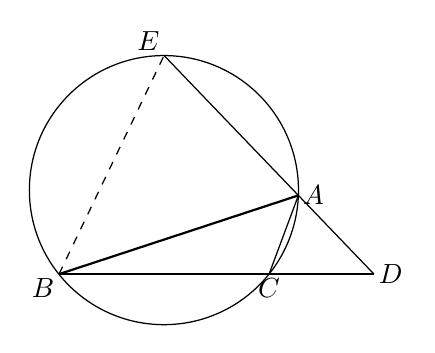
\begin{tikzpicture}[scale=1.6, line width=0.45pt,
  every node/.style={inner sep=1.5pt}]
  \coordinate (B) at (0,0);
  \coordinate (C) at (1.667,0);
  \coordinate (A) at (1.900,0.625);
  \coordinate (D) at (2.500,0);
  \coordinate (E) at (0.834,1.735);
  \draw (0.833,0.667) circle (1.068);
  \draw[line width=0.8pt] (B) -- (A);
  \draw[line width=0.8pt] (B) -- (D);
  \draw (A) -- (C);
  \draw (E) -- (D);
  \draw[dashed] (B) -- (E);
  \node[anchor=north east] at (B) {$B$};
  \node[anchor=north] at (C) {$C$};
  \node[anchor=west] at (A) {$A$};
  \node[anchor=west] at (D) {$D$};
  \node[anchor=south east] at (E) {$E$};
\end{tikzpicture}
